    \documentclass{article}
%------------------------- packages -------------------------%
\usepackage[vietnamese.licr]{babel}
\usepackage{listings}
\usepackage{tvietlistings}
\usepackage[T1]{fontenc}
\usepackage[utf8]{inputenc} % Đảm bảo sử dụng mã hóa UTF-8
\usepackage{float}
\usepackage[many]{tcolorbox}
\usepackage[unicode,hidelinks]{hyperref}    % for reference
\usepackage{geometry}   % for layout
\usepackage{amsmath}    % for math
\usepackage{xcolor}     % for color
% for figure
\usepackage{graphicx}
\usepackage{caption}    
% for code
\usepackage{minted}
\usepackage[normalem]{ulem}
% for table
\usepackage{xparse}
\usepackage{float}      
\usepackage{paracol}
\usepackage{array}
\usepackage{multirow}
% for header & footer 
\usepackage{fancyhdr}
\usepackage{lastpage}
\usepackage{CJKutf8}
\usepackage{xcolor}


%------------------------- set up -------------------------%
% figure
\graphicspath{{./Images/}}              % path to image
\captionsetup[figure]{labelfont={small,bf,it},textfont={small,it}}
% paragraph
\setlength{\parindent}{0pt}
\setlength{\parskip}{12pt}
\setlength{\parskip}{6pt}               % disables indentation
\renewcommand{\baselinestretch}{1.5}    % line spacing

% code
\def\code#1{\texttt{#1}}    % font
\usemintedstyle{vs}         % minted theme
\setminted{
    autogobble,             % remove all common leading whitespace
    baselinestretch=1.0,
    bgcolor=gray!5!white,
    breaklines,
    %linenos,               % enables line numbers
    fontsize=\footnotesize
}
% Table addrow Macro with dyanamic
% Define the new addrow command to accept a variable number of arguments
\NewDocumentCommand{\addrow}{>{\SplitList{;}}m}{%
  \processline#1\relax
}


% Define a custom style
\lstdefinestyle{myStyle}{
    frame=l,
    framesep=4.5mm,
    framexleftmargin=2.5mm,
    basicstyle=\ttfamily\footnotesize,
    captionpos=b,
    commentstyle=\color{comment},
    breakatwhitespace=false,         
    breaklines=true,                 
    keepspaces=true,                 
    numbers=left,       
    numbersep=5pt,                  
    showspaces=false,                
    showstringspaces=false,
    showtabs=false,                  
    tabsize=2,
    keywords={if, else, for, while, repeat, function, in, next, break, library, ifelse, select, return, print, mutate, hist, tapply, apply, sapply, boxplot, barplot, factor},
		% keywordstyle=\color{blue}\bfseries,
        keywordstyle=\color{comment},
		ndkeywords={class, data.frame, numeric, matrix, character, list, c, seq},
		ndkeywordstyle=\color{black}\bfseries,
		identifierstyle=\color{black},
		sensitive=false,
		comment=[l]{\#},
}
% Helper macro to process each item
\newcommand{\processline}[1]{%
  \ifx\relax#1\relax % End of the list
    \\ \hline
  \else
    #1%
    \expandafter\processnext
  \fi
}

\newcommand{\processnext}[1]{%
  \ifx\relax#1\relax % End of the list
    \\ \hline
  \else
    & #1%
    \expandafter\processnext
  \fi
}

% Callout
\definecolor{main}{HTML}{5989cf}    % setting main color to be used
\definecolor{comment}{HTML}{606060}
\definecolor{sub}{HTML}{cde4ff}     % setting sub color to be used
\newtcolorbox{boxH}{
    % fontupper = \bf,
    boxrule = 1.5pt,
    colback = white, 
    colframe = black % frame color
}
% End
%------------------------- layout & margin -------------------------%
\geometry{
    a4paper,        % redundant if already in \documentclass
    left=20.32mm,
    right=20.32mm,
    top=25.40mm,
    bottom=25.40mm,
    heightrounded,  % better use it
}
\setlength{\parindent}{20pt}
%------------------------- header & footer -------------------------%
\renewcommand{\headrulewidth}{0.5pt}
\renewcommand{\footrulewidth}{0.5pt}
\setlength{\headheight}{24.5pt}
\pagestyle{fancy}

\fancyhead{}    % clear all header fields
\fancyhead[L]{
    \begin{tabular}{ll}
        \begin{picture}(10,10)
            \put(0,-7){
\includegraphics[width=8mm]{{Images/bachkhoa_logo.png}}}
        \end{picture}&
    	\begin{tabular}{l}
    	    {\ttfamily Trường Đại học Bách Khoa Tp. Hồ Chí Minh} \\
    	    {\ttfamily Khoa Khoa học và Kỹ thuật Máy tính} \\
    	\end{tabular} 	
    \end{tabular}
}

\fancyfoot{}    % clear all footer fields
\fancyfoot[L]{\footnotesize {\ttfamily Báo cáo Hệ Quản Trị Cơ Sở Dữ Liệu}}
\fancyfoot[R]{\footnotesize {\ttfamily Trang {\thepage}/\pageref{LastPage}}}
% might change to \scriptsize

%------------------------- body -------------------------%
\begin{document}


% Use \lstset to make myStyle the global default
\lstset{style=myStyle}
%-------------------- cover --------------------%
\begin{titlepage}
\begin{center}
    \large ĐẠI HỌC QUỐC GIA THÀNH PHỐ HỒ CHÍ MINH \\
    TRƯỜNG ĐẠI HỌC BÁCH KHOA \\
    KHOA KHOA HỌC VÀ KỸ THUẬT MÁY TÍNH
\end{center}

\vspace{1.5cm}

\begin{figure}[!ht]
    \centering 
\includegraphics[width=3.5cm]{Images/bachkhoa_logo.png}
\end{figure}

\begin{table}[H]
    \centering
    \begin{tabular}{c}
    {\bf \Large HỆ QUẢN TRỊ CƠ SỞ DỮ LIỆU (CO3021)} \\ \\
    \hline  \\
    \multicolumn{0}{c}{{\bf \huge Báo cáo Bài tập lớn}} \\
    {\bf \huge Postgres và MongoDB}     \\  
    \\
    \hline
    \end{tabular}
\end{table}

\begin{table}[h]
\centering
\begin{tabular}{lrlc}

\hspace{5 cm} & Giáo viên hướng dẫn: & LÊ THỊ BẢO THU\\
& Các thành viên nhóm &  
 	
    Đào Duy Tùng& 2033364\\
& & Huỳnh Huynh Mân & 2033364\\
& & Vũ Trường Khoa& 2252867\\
& & Tôn Trọng Tín & 2333464\\
\end{tabular}
\textbf{\textit{}}\end{table}

\vspace{1.0cm}

\begin{center}
    \footnotesize Tp. Hồ Chí Minh, Tháng 03/2025
\end{center}
\end{titlepage}
\newpage
%-------------------- mission --------------------%
%\renewcommand{\arraystretch}{2}

%-------------------- mục lục --------------------%
\tableofcontents
%-------------------- Chia các mục --------------------%
\section*{\begin{center}
\Huge{Giới thiệu}
\end{center}}
\begin{itemize}
    \item Mục tiêu:
    \begin{itemize}
        \item So sánh sự khác biệt giữa Postgres (CSDL quan hệ) và MongoDB (CSDL NoSQL dạng document) theo các khía cạnh: lưu trữ \& quản lý dữ liệu, indexing, xử lý truy vấn, giao dịch, kiểm soát đồng thời, sao lưu \& phục hồi dữ liệu.
        \item Minh họa bằng các ví dụ code cụ thể cho từng loại hình cũng như nêu ra các loại (types) hay phương pháp mà mỗi hệ thống hỗ trợ.
    \end{itemize}
    \item Lý do chọn đề tài:
    \begin{itemize}
        \item Giúp hiểu rõ ưu, nhược điểm của hai hệ thống để lựa chọn phù hợp với yêu cầu ứng dụng thực tế.
        \item Cung cấp cơ sở cho việc xây dựng ứng dụng demo, ví dụ: ứng dụng thương mại điện tử đơn giản trên MongoDB thể hiện các khía cạnh đã nêu.
    \end{itemize}
\end{itemize}

\noindent
Trong quá trình hiện thực và báo cáo, nếu có vấn đề sai sót, nhóm rất mong nhận được ý kiến đóng góp từ thầy và các bạn để hoàn thiện hơn.


\newpage

\section{Giới thiệu tổng quan}
\subsection{Các khái niệm cơ bản}
\subsubsection{Cơ sở dữ liệu quan hệ (Relational Database)}

\textbf{Khái niệm}

Là hệ thống quản lý cơ sở dữ liệu dựa trên mô hình bảng, trong đó dữ liệu được lưu trữ dưới dạng các bảng có các hàng (record) và cột (field). Các bảng có thể liên kết với nhau thông qua các mối quan hệ (relationship) như khóa chính (primary key) và khóa ngoại (foreign key).

\noindent
\textbf{Đặc điểm}
\begin{itemize}
    \item \textbf{Schema cố định}: Cần định nghĩa cấu trúc dữ liệu trước khi lưu trữ.
    \item \textbf{Ngôn ngữ truy vấn}: Sử dụng SQL (Structured Query Language) để thao tác dữ liệu.
    \item \textbf{Tính nhất quán cao}: Hỗ trợ giao dịch theo chuẩn ACID (Atomicity, Consistency, Isolation, Durability).
    \item \textbf{Ví dụ}: PostgreSQL, MySQL, Oracle.
\end{itemize}



\subsubsection{Cơ sở dữ liệu NoSQL dạng document (Document-oriented NoSQL Database)}

\textbf{Khái niệm}

Là hệ thống quản lý cơ sở dữ liệu NoSQL, lưu trữ dữ liệu dưới dạng các tài liệu (documents) thường ở định dạng JSON, BSON hoặc XML. Mỗi tài liệu có thể chứa các cấu trúc dữ liệu phức tạp và không cần phải tuân theo một schema cố định.

\noindent
\textbf{Đặc điểm}
\begin{itemize}
    \item \textbf{Schema linh hoạt}: Cho phép lưu trữ dữ liệu với cấu trúc khác nhau trong cùng một collection.
    \item \textbf{Khả năng mở rộng}: Dễ dàng mở rộng theo chiều ngang (scaling out) để xử lý khối lượng dữ liệu lớn.
    \item \textbf{Truy vấn qua API hoặc ngôn ngữ truy vấn riêng}: Sử dụng cú pháp truy vấn đặc thù như MongoDB Query Language (MQL).
    \item \textbf{Ví dụ}: MongoDB, CouchDB.
\end{itemize}

\newpage

\subsection{PostgreSQL là gì?}

\textbf{PostgreSQL} là một hệ quản trị cơ sở dữ liệu quan hệ (RDBMS) mã nguồn mở mạnh mẽ, nổi tiếng với tính tuân thủ chuẩn SQL, tính năng mở rộng cao và hỗ trợ đầy đủ các giao dịch ACID. Nó được thiết kế để xử lý khối lượng công việc phức tạp, hỗ trợ nhiều kiểu dữ liệu (bao gồm JSON, XML) và cung cấp nhiều tính năng tiên tiến như MVCC (Multi-Version Concurrency Control), stored procedures, trigger, và hỗ trợ lập trình mở rộng qua các ngôn ngữ như PL/pgSQL, Python,…

\subsubsection{Khi nào nên dùng PostgreSQL?}

\begin{itemize}
    \item \textbf{Ứng dụng đòi hỏi tính toàn vẹn và nhất quán cao}: Khi ứng dụng cần đảm bảo các giao dịch tuân thủ chuẩn ACID (Atomicity, Consistency, Isolation, Durability), chẳng hạn như các hệ thống tài chính, ngân hàng, hay quản lý đơn hàng.
    \item \textbf{Yêu cầu xử lý truy vấn phức tạp}: PostgreSQL rất mạnh mẽ với các truy vấn liên quan đến join, subquery, aggregate… Điều này phù hợp với các hệ thống phân tích, báo cáo và truy vấn dữ liệu phức tạp.
    \item \textbf{Định nghĩa schema rõ ràng}: Khi dữ liệu có cấu trúc xác định và cần quản lý bằng các ràng buộc như khóa chính, khóa ngoại, unique, check constraints để đảm bảo tính hợp lệ của dữ liệu.
    \item \textbf{Tính mở rộng theo chiều dọc}: Ứng dụng cần tận dụng tài nguyên của một máy chủ mạnh (CPU, RAM, ổ đĩa) để xử lý khối lượng lớn giao dịch.
    \item \textbf{Hỗ trợ đa dạng kiểu dữ liệu và mở rộng}: Khi cần lưu trữ các kiểu dữ liệu phức tạp như JSON hoặc các kiểu dữ liệu địa lý, PostgreSQL cung cấp các module như PostGIS cho dữ liệu không gian.
\end{itemize}

\subsubsection{Khi nào không nên dùng PostgreSQL?}

\begin{itemize}
    \item \textbf{Ứng dụng yêu cầu mở rộng theo chiều ngang cực lớn}: Nếu hệ thống cần mở rộng qua nhiều máy chủ để xử lý khối lượng dữ liệu khổng lồ (big data) với khả năng phân mảnh (sharding) tự động, một số cơ sở dữ liệu NoSQL hoặc hệ thống NewSQL có thể phù hợp hơn.
    \item \textbf{Yêu cầu hiệu năng cao cho các tác vụ đơn giản, không cần giao dịch phức tạp}: Trong các ứng dụng chỉ cần xử lý các thao tác đọc/ghi đơn giản, với yêu cầu linh hoạt về schema (ví dụ: lưu trữ log, dữ liệu không cấu trúc) thì các hệ thống như MongoDB hoặc các cơ sở dữ liệu key-value có thể là lựa chọn tối ưu hơn.
    \item \textbf{Độ phức tạp quản trị}: Mặc dù PostgreSQL rất mạnh mẽ, nhưng với các ứng dụng nhỏ hoặc không đòi hỏi các tính năng nâng cao, cấu hình và quản trị của PostgreSQL có thể phức tạp hơn so với một số hệ thống nhẹ hơn.
\end{itemize}

\textbf{PostgreSQL} là lựa chọn tuyệt vời cho các ứng dụng yêu cầu tính nhất quán, xử lý giao dịch phức tạp và truy vấn dữ liệu mạnh mẽ. Tuy nhiên, nếu hệ thống cần mở rộng theo chiều ngang quy mô lớn hoặc không cần nhiều tính năng phức tạp, các lựa chọn khác như NoSQL hoặc cơ sở dữ liệu key-value có thể là giải pháp hợp lý hơn.


\subsection{MongoDB là gì?}

\textbf{MongoDB} là một hệ quản trị cơ sở dữ liệu NoSQL dạng document, nghĩa là nó lưu trữ dữ liệu dưới dạng các tài liệu (documents) – thường ở định dạng JSON hoặc BSON – trong các collection. Điều này mang lại sự linh hoạt cao vì không cần phải định nghĩa một schema cứng nhắc trước khi lưu trữ dữ liệu.



\subsubsection{Khi nào nên dùng MongoDB?}
\begin{itemize}
    \item \textbf{Ứng dụng cần tính linh hoạt về dữ liệu}: Khi dữ liệu có thể thay đổi cấu trúc theo thời gian hoặc khi dữ liệu có tính chất phi cấu trúc. Ví dụ: các ứng dụng nội dung, blog, hoặc lưu trữ log, nơi mỗi bản ghi có thể có các thuộc tính khác nhau.
    \item \textbf{Khả năng mở rộng theo chiều ngang}: MongoDB được thiết kế để dễ dàng phân mảnh (sharding) và mở rộng qua nhiều máy chủ, phù hợp với các ứng dụng cần xử lý khối lượng dữ liệu lớn hoặc cần tăng tốc độ xử lý bằng cách phân phối tải.
    \item \textbf{Phát triển nhanh và linh hoạt}: Trong các dự án yêu cầu phát triển nhanh, không muốn ràng buộc dữ liệu với schema cứng nhắc, MongoDB cho phép thay đổi cấu trúc dữ liệu dễ dàng trong quá trình phát triển.
    \item \textbf{Ứng dụng thời gian thực}: Các ứng dụng cần hiệu năng ghi/đọc cao, ví dụ như các dịch vụ web, hệ thống theo dõi (monitoring) hay trò chuyện trực tuyến, có thể hưởng lợi từ kiến trúc NoSQL của MongoDB.
\end{itemize}

\subsubsection{Khi nào không nên dùng MongoDB?}

\begin{itemize}
    \item \textbf{Yêu cầu giao dịch phức tạp và tính nhất quán cao}: Nếu ứng dụng cần thực hiện các giao dịch phức tạp với tính toàn vẹn dữ liệu nghiêm ngặt (ACID) như trong hệ thống tài chính hoặc ngân hàng, các cơ sở dữ liệu quan hệ như PostgreSQL thường phù hợp hơn.
    \item \textbf{Các phép join và truy vấn liên quan đến dữ liệu có mối quan hệ chặt chẽ}: MongoDB không hỗ trợ join giữa các collection một cách tự nhiên như SQL. Nếu dữ liệu có nhiều mối liên kết phức tạp cần join, thì hệ thống CSDL quan hệ sẽ có lợi thế hơn.
    \item \textbf{Yêu cầu xử lý truy vấn phức tạp}: Khi ứng dụng cần thực hiện các truy vấn phân tích và tổng hợp phức tạp, các hệ thống RDBMS thường có optimizer mạnh mẽ và cú pháp SQL hỗ trợ tốt hơn.
\end{itemize}

\textbf{MongoDB} là một giải pháp tuyệt vời cho các ứng dụng cần sự linh hoạt trong lưu trữ dữ liệu, khả năng mở rộng theo chiều ngang và tốc độ xử lý nhanh cho các tác vụ ghi/đọc đơn giản. Tuy nhiên, nếu ứng dụng của bạn đòi hỏi tính toàn vẹn dữ liệu cao, giao dịch phức tạp, hoặc các phép toán liên quan đến nhiều mối quan hệ dữ liệu (join), một hệ quản trị cơ sở dữ liệu quan hệ (như PostgreSQL) có thể là lựa chọn phù hợp hơn.
\newpage

\section{Nội dung phân tích}

\subsection{Data Storage \& Management}

\subsubsection{Postgres}

\begin{itemize}
    \item \textbf{Đặc điểm}:
    \begin{itemize}
        \item Dữ liệu được lưu trữ trong các bảng với cấu trúc (schema) cố định.
        \item Ràng buộc kiểu dữ liệu, khóa chính, khóa ngoại, ... giúp đảm bảo tính nhất quán.
    \end{itemize}
    \item \textbf{Ví dụ Code (SQL)}: 
        \begin{lstlisting}[language=sql]
CREATE TABLE users (
    id SERIAL PRIMARY KEY,
    name VARCHAR(100) NOT NULL,
    email VARCHAR(100) UNIQUE NOT NULL
);\end{lstlisting}
\end{itemize}

\noindent
\subsubsection{MongoDB}

\begin{itemize}
    \item \textbf{Đặc điểm}:
    \begin{itemize}
        \item Dữ liệu được lưu dưới dạng document (JSON/BSON) trong các collection.
        \item Schema linh hoạt, dễ dàng mở rộng với dữ liệu phi cấu trúc.
    \end{itemize}
    \item \textbf{Ví dụ Code (Mongo Shell)}: 
        \begin{lstlisting}[language=java]
db.users.insertOne({
    name: "John Doe",
    email: "john.doe@example.com"
});\end{lstlisting}
\end{itemize}

\subsubsection{So sánh}
\begin{itemize}
    \item \textbf{Schema cố định so sánh linh hoạt}: \textbf{Postgres} yêu cầu định nghĩa cấu trúc dữ liệu trước, còn \textbf{MongoDB} cho phép lưu trữ dữ liệu không đồng nhất.
    \item \textbf{Quản lý dữ liệu}: Các ràng buộc (constraints) mạnh mẽ của \textbf{Postgres} hỗ trợ tính toàn vẹn dữ liệu, trong khi \textbf{MongoDB} cung cấp tính mở rộng dễ dàng.
\end{itemize}

\newpage
\subsection{Indexing}

Indexing là một cơ chế tối ưu hóa trong cơ sở dữ liệu, hoạt động như “mục lục” của một cuốn sách, giúp hệ thống định vị và truy xuất dữ liệu một cách nhanh chóng.

\subsubsection{Mục đích sử dụng Indexing}

\begin{itemize}
    \item \textbf{Tăng tốc độ truy vấn}: Index giúp hệ thống tìm kiếm các bản ghi mà không cần quét toàn bộ bảng (full table scan). Điều này đặc biệt quan trọng với các bảng chứa hàng triệu bản ghi.
    \item \textbf{Tối ưu hóa hiệu suất}: Khi truy vấn có điều kiện (WHERE, JOIN, ORDER BY, GROUP BY), index cho phép truy vấn truy cập dữ liệu theo cách đã được sắp xếp và tối ưu, giảm tải cho CPU và I/O.
\end{itemize}

\subsubsection{Khi nào nên sử dụng Indexing}

\begin{itemize}
    \item \textbf{Bảng dữ liệu lớn}: Với bảng có số lượng bản ghi lớn, index giúp cải thiện thời gian truy vấn một cách đáng kể.
    \item \textbf{Truy vấn có điều kiện thường xuyên}: Nếu các truy vấn của bạn thường tìm kiếm theo một hoặc vài cột cụ thể, việc tạo index trên những cột này sẽ tăng tốc độ tìm kiếm.
    \item \textbf{Truy vấn sắp xếp và nhóm dữ liệu}: Các câu lệnh sử dụng ORDER BY hoặc GROUP BY có thể được tối ưu khi có index phù hợp.
\end{itemize}

\subsubsection{Khi nào không nên sử dụng Indexing}

\begin{itemize}
    \item \textbf{Bảng dữ liệu nhỏ}: Với bảng chứa ít bản ghi, lợi ích của việc sử dụng index không đáng kể vì chi phí duy trì index có thể vượt quá lợi ích cải thiện tốc độ truy vấn.
    \item \textbf{Thao tác ghi dữ liệu nhiều}: Index không chỉ cải thiện truy vấn mà còn cần được cập nhật mỗi khi có INSERT, UPDATE hoặc DELETE. Trong các bảng có tần suất ghi/chỉnh sửa cao, nhiều index có thể làm chậm hiệu năng ghi dữ liệu.
    \item \textbf{Quá nhiều index trên một bảng}: Việc tạo quá nhiều index có thể dẫn đến việc quản lý và cập nhật index trở nên nặng nề, làm giảm hiệu suất của các thao tác ghi.
\end{itemize}

Tóm lại, \textbf{index} là công cụ mạnh mẽ để tối ưu hóa truy vấn, nhưng cần được áp dụng một cách hợp lý để tránh tác động tiêu cực đến hiệu năng ghi dữ liệu.

\newpage
\subsubsection{Postgres}

\begin{itemize}
    \item Các loại index hỗ trợ:
    \begin{itemize}
        \item \textbf{B-tree}: Mặc định cho hầu hết các loại truy vấn.
        \item \textbf{Hash, GiST, GIN, SP-GiST}: Dùng cho các trường hợp đặc thù như tìm kiếm văn bản, dữ liệu không gian, …
    \end{itemize}
    \item Ví dụ Code (SQL):\begin{lstlisting}[language=sql]
-- Tạo B-tree index trên cột email
CREATE INDEX idx_users_email ON users(email);\end{lstlisting}
\end{itemize}

\subsubsection{MongoDB}

\begin{itemize}
    \item Các loại index hỗ trợ:
    \begin{itemize}
        \item \textbf{Single Field Index}: Index trên một trường.
        \item \textbf{Compound Index}: Index trên nhiều trường.
        \item \textbf{Text Index}: Dành cho tìm kiếm văn bản.
        \item \textbf{Geospatial Index}: Dành cho dữ liệu không gian.
    \end{itemize}
    \item Ví dụ Code (Mongo Shell):\begin{lstlisting}[language=sql]
// Tạo index trên trường email
db.users.createIndex({ email: 1 });
\end{lstlisting}
\end{itemize}

\subsubsection{So sánh}

\begin{itemize}
    \item \textbf{Đa dạng index}: Postgres có nhiều loại index phục vụ cho các mục đích tối ưu hóa phức tạp, trong khi MongoDB tập trung vào các loại index hỗ trợ nhanh cho việc tìm kiếm theo document.
    \item \textbf{Cách triển khai}: Cách định nghĩa index khá khác nhau giữa SQL và JSON-like query language.
\end{itemize}
\newpage
\subsection{Query Processing}

\textbf{Query Processing} (Xử lý truy vấn) là quá trình chuyển đổi câu lệnh truy vấn do người dùng nhập (ví dụ: SQL trong các cơ sở dữ liệu quan hệ hay MQL trong MongoDB) thành một kế hoạch thực thi hiệu quả để truy xuất dữ liệu từ cơ sở dữ liệu. 

\textbf{Query processing} (xử lý truy vấn) là một quy trình phức tạp trong hệ thống cơ sở dữ liệu, bao gồm các bước từ khi nhận truy vấn từ người dùng đến khi trả về kết quả. Quy trình này đóng vai trò then chốt, quyết định hiệu suất và độ tin cậy của hệ thống cơ sở dữ liệu.

\textbf{Query processing} là chuỗi các hoạt động xử lý truy vấn trong hệ thống cơ sở dữ liệu, bao gồm:

\begin{itemize}
    \item Phân tích cú pháp truy vấn
    \item Kiểm tra tính hợp lệ
    \item Tối ưu hóa truy vấn
    \item Tạo kế hoạch thực thi
    \item Thực thi truy vấn
    \item Tổng hợp và trả về kết quả
\end{itemize}

\noindent
\textbf{Vai trò và Lợi ích của Query Processing}

\begin{itemize}
    \item Tăng hiệu năng truy xuất dữ liệu:
    \begin{itemize}
        \item Giúp giảm thiểu thời gian truy vấn thông qua tối ưu hóa kế hoạch thực thi.
    \end{itemize}
    \item Quản lý tài nguyên hiệu quả:
    \begin{itemize}
        \item Giúp hệ thống sử dụng CPU, bộ nhớ và I/O một cách hợp lý, tránh việc quét toàn bộ bảng không cần thiết.
    \end{itemize}
    \item Hỗ trợ truy vấn phức tạp:
    \begin{itemize}
        \item Cho phép xử lý các truy vấn có nhiều phép toán như join, subquery, aggregate… một cách hiệu quả.
    \end{itemize}
\end{itemize}

\textbf{Query Processing} đóng vai trò quan trọng trong việc đảm bảo rằng hệ thống cơ sở dữ liệu thực thi các truy vấn một cách nhanh chóng và hiệu quả, góp phần nâng cao hiệu năng tổng thể của ứng dụng.

\newpage

\subsubsection{Postgres}

PostgreSQL là một hệ quản trị cơ sở dữ liệu quan hệ mã nguồn mở với kiến trúc xử lý truy vấn phức tạp và hiệu quả.

Dưới đây là mô hình hoạt động của query processing trong PostgreSQL:

\begin{tikzpicture}[node distance=0.5cm and 0.5cm, auto,
    block/.style={rectangle, draw, text centered, rounded corners},
    line/.style={draw, -Latex}]

  % Main flow nodes
  \node (sql) [block] {SQL Query};
  \node (parser) [block, right=of sql] {Parser};
  \node (analyzer) [block, right=of parser] {Analyzer};
  \node (rewriter) [block, right=of analyzer] {Rewriter};
  \node (optimizer) [block, right=of rewriter] {Planner/Optimizer};
  \node (executor) [block, right=of optimizer] {Executor};
  \node (results) [block, right=of executor] {Results};

  % Feedback loop nodes
  \node (catalog) [block, below=1.5cm of analyzer] {Catalog};
  \node (rules) [block, below=1.5cm of rewriter] {Rule System};
  \node (stats) [block, below=1.5cm of optimizer] {Statistics};

  % Arrows for the main flow
  \draw [line] (sql) -- (parser);
  \draw [line] (parser) -- (analyzer);
  \draw [line] (analyzer) -- (rewriter);
  \draw [line] (rewriter) -- (optimizer);
  \draw [line] (optimizer) -- (executor);
  \draw [line] (executor) -- (results);

  % Arrows for the feedback loops
  \draw [line] (rules) -- (rewriter);
  \draw [line] (catalog) -- (analyzer); % Feedback to Analyzer
  \draw [line] (stats) -- (optimizer); % Feedback to Optimizer

\end{tikzpicture}


Quá trình này bao gồm một số bước chính:

\begin{enumerate}
    \item \textbf{Parser (Bộ phân tích cú pháp)}:
    \begin{itemize}
        \item Phân tích câu truy vấn để kiểm tra tính hợp lệ về cú pháp và đảm bảo rằng các từ khóa, tên bảng, tên trường, … được viết đúng theo quy tắc của ngôn ngữ truy vấn.
        \item Trình phân tích cú pháp truy vấn phân tích cấu trúc cú pháp của truy vấn, đảm bảo nó tuân thủ các quy tắc ngữ pháp của ngôn ngữ PostgreSQL. Nó kiểm tra lỗi, xác thực cấu trúc truy vấn và tạo cây phân tích cú pháp. Đầu ra là một cây phân tích cú pháp : 

      \begin{figure}[H]
                    \centering
                    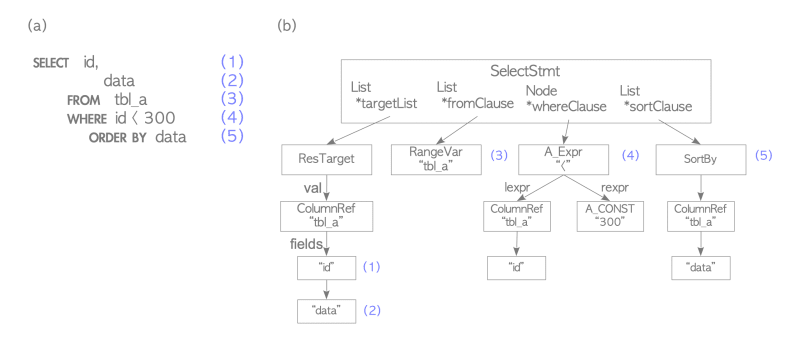
\includegraphics[width = 1\textwidth]{Images/query-progress-01.png}
                    \caption{Ví dụ cây phân tích cú pháp}
                \end{figure}
                
    \end{itemize}
     \item \textbf{Semantic Analysis}:
    \begin{itemize}
        \item  Sau khi phân tích cú pháp thành công, trình phân tích ngữ nghĩa (semantic analyzer) sẽ kiểm tra ý nghĩa của câu truy vấn. Nó xác minh sự tồn tại của các bảng, cột, hàm và các đối tượng cơ sở dữ liệu khác được tham chiếu trong truy vấn. Nó cũng kiểm tra quyền truy cập của người dùng để đảm bảo họ có quyền thực hiện truy vấn.
        \item Kiểm tra tính hợp lệ của truy vấn
        \item Xác minh rằng các bảng, cột và hàm được tham chiếu tồn tại
        \item Phân giải các tên cột và kiểm tra quyền truy cập
        \item Chuyển đổi parse tree thành query tree
        \item Xác định kiểu dữ liệu cho mỗi biểu thức
    \end{itemize}
    \item \textbf{Query Rewriting (Chuyển đổi truy vấn)}:
    \begin{itemize}
        \item Giai đoạn này có thể xảy ra nếu có các quy tắc (rules) hoặc view được định nghĩa. Trình viết lại (rewriter) có thể sửa đổi câu truy vấn ban đầu dựa trên các quy tắc này để tối ưu hóa hoặc thực hiện các logic phức tạp.
        \item Biến đổi câu truy vấn ban đầu thành dạng dễ tối ưu hóa hơn, chẳng hạn như đơn giản hóa các biểu thức logic hoặc chuyển đổi cấu trúc của câu truy vấn.
        \item Áp dụng các quy tắc từ hệ thống rules
        \item Mở rộng view thành các truy vấn trên bảng cơ sở
        \item Áp dụng các ràng buộc bảo mật (Row-Level Security)
        \item Xử lý các trigger và policy
    \end{itemize}
    \item \textbf{Planner/Optimizer (Bộ lập kế hoạch/tối ưu hóa)}:
    \begin{itemize}
        \item Đây là giai đoạn quan trọng nhất. Trình lập kế hoạch (planner) sẽ tạo ra nhiều kế hoạch thực thi khác nhau cho cùng một câu truy vấn. Mỗi kế hoạch này bao gồm các bước cụ thể để truy cập và xử lý dữ liệu, chẳng hạn như sử dụng index, thực hiện sequential scan, hoặc chọn thuật toán join phù hợp.
        \item PostgreSQL sẽ tạo kế hoạch thực thi (execution plan) bằng cách chọn phương án tối ưu nhất dựa trên các chỉ mục và thống kê dữ liệu. Điều này bao gồm việc quyết định thứ tự thực thi các bước trong truy vấn.
        \item Xác định kế hoạch thực thi tối ưu bằng cách cân nhắc nhiều phương án khác nhau. Hệ quản trị cơ sở dữ liệu sẽ dựa vào các thống kê dữ liệu, cấu trúc bảng, chỉ mục, … để lựa chọn chiến lược tốt nhất nhằm giảm thiểu thời gian và tài nguyên cần thiết cho truy vấn.
        \item Trình tối ưu hóa (optimizer) sẽ đánh giá chi phí ước tính của mỗi kế hoạch thực thi được tạo ra bởi trình lập kế hoạch. Chi phí này thường được tính toán dựa trên các yếu tố như thời gian thực thi dự kiến, số lượng I/O cần thiết và mức sử dụng tài nguyên hệ thống. Trình tối ưu hóa sẽ chọn kế hoạch có chi phí thấp nhất để thực thi.
        \item Phân tích nhiều kế hoạch thực thi có thể
        \item Ước tính chi phí cho mỗi kế hoạch dựa trên thống kê
        \item Lựa chọn kế hoạch có chi phí thấp nhất
        \item Xác định chiến lược quét (table scan, index scan)
        \item Quyết định phương pháp join (nested loop, hash join, merge join)
        \item Tối ưu hóa các phép lọc và sắp xếp
    \end{itemize}
    \item \textbf{Query Execution (Thực thi truy vấn)}:
    \begin{itemize}
        \item Thực hiện kế hoạch truy vấn đã được tối ưu hóa, truy xuất dữ liệu từ các bảng hoặc collections theo cách hiệu quả nhất.
    \end{itemize}
    \item \textbf{Formatting (Định dạng kết quả)}:
    \begin{itemize}
        \item Sau khi truy xuất dữ liệu, kết quả được định dạng lại và trả về cho người dùng hoặc ứng dụng theo yêu cầu.
    \end{itemize}
\end{enumerate}

\textbf{Đặc điểm} : 
\begin{itemize}
    \item Sử dụng SQL, hỗ trợ  các truy vấn phức tạp như join, subquery, aggregate.
    \item Có query optimizer mạnh mẽ giúp tối ưu thời gian thực thi.
\end{itemize}

\textbf{Ví dụ Code (SQL)}:

\begin{lstlisting}[style=sql, caption=Ví dụ query trong Postgres, label=sql:example]
SELECT u.name, o.order_date
FROM users u
JOIN orders o ON u.id = o.user_id
WHERE u.email = 'john.doe@example.com';
\end{lstlisting}


\textbf{Query Optimization trong PostgreSQL}

\textbf{Query optimization} trong PostgreSQL là quá trình tự động hoặc thủ công để cải thiện hiệu suất của các câu truy vấn SQL. Mục tiêu là giảm thiểu thời gian thực thi và tài nguyên hệ thống cần thiết.

Có nhiều kỹ thuật để tối ưu hóa truy vấn trong PostgreSQL:

\begin{enumerate}
    \item \textbf{Sử dụng Index}: Index là cấu trúc dữ liệu đặc biệt giúp PostgreSQL tìm kiếm các hàng cụ thể trong bảng một cách nhanh chóng. Tạo index trên các cột thường xuyên được sử dụng trong mệnh đề \textbf{WHERE}, \textbf{JOIN}, \textbf{ORDER BY}, và \textbf{GROUP BY}.
    \begin{itemize}
        \item \textbf{Index Optimization}: Sử dụng B-tree, Hash, GIN, GiST.
        \begin{itemize}
            \item \textbf{B-tree indexes}: Chỉ mục chuẩn cho các phép so sánh =, <, >, <=, >=:     
\begin{lstlisting}[style=sql, caption=Ví dụ sử dụng B-tree indexes trong Postgres, label=sql:example]
CREATE INDEX idx\_employee\_name ON employees(name);
\end{lstlisting}
            \item \textbf{Hash indexes} : Hiệu quả cho phép so sánh bằng.
\begin{lstlisting}[style=sql, caption=Ví dụ sử dụng Hash indexes trong Postgres, label=sql:example]
CREATE INDEX idx_employee_id_hash ON employees USING HASH (employee_id);
\end{lstlisting}
            \item \textbf{GiST indexes}: Cho dữ liệu không chuẩn (hình học, văn bản)
\begin{lstlisting}[style=sql, caption=Ví dụ sử dụng Hash indexes trong Postgres, label=sql:example]
CREATE INDEX idx_location ON stores USING GIST (location);
\end{lstlisting}
            \item \textbf{GIN indexes}: Cho dữ liệu có nhiều giá trị trong một trường (arrays, jsonb)
\begin{lstlisting}[style=sql, caption=Ví dụ sử dụng GIN indexes trong Postgres, label=sql:example]
CREATE INDEX idx_tags ON products USING GIN (tags);
\end{lstlisting}

            \item \textbf{BRIN indexes}: Cho dữ liệu có tổ chức tự nhiên (timestamps)
\begin{lstlisting}[style=sql, caption=Ví dụ sử dụng BRIN indexes trong Postgres, label=sql:example]
CREATE INDEX idx_timestamp ON logs USING BRIN (created_at);
\end{lstlisting}

            \item \textbf{Partial indexes}: Chỉ đánh chỉ mục cho một phần dữ liệu
\begin{lstlisting}[style=sql, caption=Ví dụ sử dụng Partial indexes trong Postgres, label=sql:example]
CREATE INDEX idx_active_users ON users(email) WHERE status = 'active';
\end{lstlisting}

            \item \textbf{Multi-column indexes}: Đánh chỉ mục nhiều cột
\begin{lstlisting}[style=sql, caption=Ví dụ sử dụng Multi-column indexes trong Postgres, label=sql:example]
CREATE INDEX idx_name_dept ON employees(department_id, last_name, first_name);
\end{lstlisting}
        \end{itemize}
        \item \textbf{Join Ordering}: Chọn thứ tự join tối ưu.

\begin{itemize}
    \item Chọn thứ tự join tối ưu
    \item Lựa chọn phương pháp join phù hợp (nested loop, hash, merge)
    \item Sử dụng join column indexes
    \item Tận dụng foreign keys
\end{itemize}

        \item \textbf{Parallel Query}: Thực thi song song.
        \item \textbf{WHERE Clause Optimization}

\begin{itemize}
    \item Sử dụng điều kiện có thể tận dụng các chỉ mục
    \item Tránh sử dụng các hàm trên cột được lọc
    \item Tận dụng phép lọc có độ chọn lọc cao
    \item Sử dụng điều kiện IN thay vì nhiều điều kiện OR
\end{itemize}

\begin{lstlisting}[style=sql, caption=Ví dụ tối ưu WHERE Clause Optimization trong Postgres, label=sql:example]
-- Tốt
SELECT * FROM orders WHERE status IN ('pending', 'processing');

-- Kém hiệu quả
SELECT * FROM orders WHERE status = 'pending' OR status = 'processing';
\end{lstlisting}


        \item \textbf{Partition Pruning}:


\begin{itemize}
    \item Chia dữ liệu thành các phân vùng
    \item Chỉ quét các phân vùng liên quan
\end{itemize}

\begin{lstlisting}[style=sql, caption=Ví dụ Partition Pruning trong Postgres, label=sql:example]
CREATE TABLE sales (
    id SERIAL,
    sale_date DATE,
    amount NUMERIC
) PARTITION BY RANGE (sale_date);

CREATE TABLE sales_2023 PARTITION OF sales
    FOR VALUES FROM ('2023-01-01') TO ('2024-01-01');

CREATE TABLE sales_2024 PARTITION OF sales
    FOR VALUES FROM ('2024-01-01') TO ('2025-01-01');
\end{lstlisting}        
        
        \item \textbf{Materialized Views}: Lưu kết quả truy vấn thường dùng.

\begin{lstlisting}[style=sql, caption=Ví dụ Materialized Views trong Postgres, label=sql:example]
CREATE MATERIALIZED VIEW sales_summary AS
SELECT 
    date_trunc('month', sale_date) AS month,
    product_id,
    SUM(quantity) AS total_quantity,
    SUM(amount) AS total_amount
FROM sales
GROUP BY date_trunc('month', sale_date), product_id;

REFRESH MATERIALIZED VIEW sales_summary;
\end{lstlisting}   

    \end{itemize}
    
    \item \textbf{Phân tích Kế hoạch Thực thi với \textit{EXPLAIN}}: Lệnh \textbf{EXPLAIN} cho phép bạn xem kế hoạch thực thi mà PostgreSQL sẽ sử dụng cho một câu truy vấn cụ thể. Điều này giúp bạn hiểu cách PostgreSQL truy cập dữ liệu và xác định các bước có thể được tối ưu hóa. Sử dụng \textbf{EXPLAIN\_ANALYZE} để có thông tin chi tiết về thời gian thực tế của từng bước.
\begin{lstlisting}[style=sql, caption=Ví dụ sử dụng EXPLAIN trong Postgres, label=sql:example]
EXPLAIN SELECT * FROM orders WHERE order_date > '2024-01-01';
EXPLAIN ANALYZE SELECT * FROM employees 
JOIN departments ON employees.department_id = departments.id
WHERE salary > 50000;


Nested Loop  (cost=0.29..34.38 rows=11 width=242) (actual time=0.038..0.078 rows=10 loops=1)
  ->  Index Scan using employees_department_id_idx on employees  (cost=0.29..16.79 rows=11 width=122) (actual time=0.020..0.033 rows=10 loops=1)
        Filter: (salary > 50000)
  ->  Index Scan using departments_pkey on departments  (cost=0.14..1.59 rows=1 width=120) (actual time=0.003..0.003 rows=1 loops=10)
        Index Cond: (id = employees.department_id)
Planning Time: 0.362 ms
Execution Time: 0.112 ms
\end{lstlisting}
    \item \textbf{Viết Truy vấn Hiệu quả}:
      \begin{itemize}
        \item Đơn giản hóa biểu thức phức tạp
        \item Loại bỏ các subqueries không cần thiết
        \item Chuyển đổi HAVING thành WHERE khi có thể
        \item Tối ưu hóa các phép UNION, INTERSECT và EXCEPT
        \item \textbf{Chỉ chọn các cột cần thiết}: Sử dụng \textbf{SELECT column1, column2} thay vì \textbf{SELECT *}.
        \item \textbf{Sử dụng mệnh đề \textit{WHERE} hiệu quả}: Lọc dữ liệu càng sớm càng tốt.
        \item \textbf{Tránh sử dụng các hàm trên các cột đã được index trong mệnh đề \textit{WHERE}}: Điều này có thể ngăn PostgreSQL sử dụng index. Thay vào đó, hãy xem xét tạo \textbf{functional index}.
        \item \textbf{Tối ưu hóa các phép toán \textit{JOIN}}: Hiểu rõ các loại \textbf{JOIN} và sử dụng loại phù hợp. Đảm bảo các cột tham gia trong \textbf{JOIN} được index.
        \item \textbf{Hạn chế sử dụng \textit{DISTINCT}}: Nếu có thể, hãy tìm cách khác để loại bỏ các bản ghi trùng lặp.
        \item \textbf{Sử dụng \textit{LIMIT}}: Nếu bạn chỉ cần một số lượng bản ghi nhất định, hãy sử dụng \textbf{LIMIT}.
    \end{itemize}
    \item \textbf{Cập nhật Thống kê với \textit{ANALYZE}}: PostgreSQL sử dụng thống kê về dữ liệu để đưa ra các quyết định tối ưu hóa. Chạy lệnh \textbf{ANALYZE} định kỳ trên các bảng để cập nhật thống kê.
\begin{lstlisting}[style=sql, caption=Ví dụ sử dụng ANALYZE trong Postgres, label=sql:example]
ANALYZE customers;
\end{lstlisting}

    \item \textbf{pg\_stat\_statements} : Theo dõi thống kê thực thi truy vấn

\begin{lstlisting}[style=sql, caption=Ví dụ theo dõi thống kê thực thi trong Postgres, label=sql:example]
SELECT query, calls, total_exec_time, rows, mean_exec_time
FROM pg_stat_statements
ORDER BY total_exec_time DESC
LIMIT 10;
\end{lstlisting}

    \item \textbf{auto\_explain} : Tự động ghi lại kế hoạch thực thi của các truy vấn chậm

\begin{lstlisting}[style=sql, caption=Ví dụ theo dõi truy vấn chậm trong Postgres, label=sql:example]
LOAD 'auto_explain';
SET auto_explain.log_min_duration = '100ms';
SET auto_explain.log_analyze = true;
\end{lstlisting}

    
    
    \item \textbf{Tối ưu hóa Cấu trúc Bảng}: Thiết kế bảng với các kiểu dữ liệu phù hợp và cân nhắc việc phân vùng bảng cho các bảng lớn.
    \item \textbf{Cấu hình PostgreSQL}: Điều chỉnh các tham số cấu hình như \textbf{shared\_buffers}, \textbf{work\_mem} có thể ảnh hưởng đến hiệu suất truy vấn.

    \begin{itemize}
        \item shared\_buffers: 25\% của RAM hệ thống
        \item effective\_cache\_size: 75\% của RAM hệ thống
        \item work\_mem: 4MB-64MB tùy ứng dụng
        \item maintenance\_work\_mem: 64MB-256MB
        \item checkpoint\_timeout: 15-30 phút
        \item default\_statistics\_target: 100-1000
    \end{itemize}
    
\end{enumerate}

\subsubsection{MongoDB}

\textbf{MongoDB} là một hệ quản trị cơ sở dữ liệu NoSQL, hướng tài liệu. Quá trình xử lý truy vấn trong MongoDB khác biệt so với PostgreSQL do sự khác biệt trong mô hình dữ liệu và ngôn ngữ truy vấn.

MongoDB xử lý truy vấn theo kiến trúc khác với cơ sở dữ liệu quan hệ do tính chất NoSQL và lưu trữ dữ liệu dạng document.

\textbf{\textit{Mô hình Query Processing trong MongoDB}}

\noindent{}
\begin{tikzpicture}[node distance=0.2cm and 0.2cm, auto,
    block/.style={rectangle, draw, text centered, rounded corners},
    line/.style={draw, -Latex}]

  % Main flow nodes
  \node (request) [block] {Client Request};
  \node (router) [block, right=of request] {Query Router};
  \node (planner) [block, right=of router] {Query Planner};
  \node (index) [block, right=of planner] {Index Selection};
  \node (execute) [block, right=of index] {Query Execution};
  \node (merge) [block, right=of execute] {Results Merging};
  \node (response) [block, right=of merge] {Response};

  % Feedback loop nodes
  \node (sharding) [block, below=0.5cm of router] {Sharding};
  \node (stats) [block, below=0.5cm of planner] {Collection Stats};
  \node (indexes) [block, below=0.5cm of index] {Indexes};

  % Arrows for the main flow
  \draw [line] (request) -- (router);
  \draw [line] (router) -- (planner);
  \draw [line] (planner) -- (index);
  \draw [line] (index) -- (execute);
  \draw [line] (execute) -- (merge);
  \draw [line] (merge) -- (response);


  % Upward arrows for feedback
  \draw [line] (sharding) -- (router);
  \draw [line] (stats) -- (planner);
  \draw [line] (indexes) -- (index);

\end{tikzpicture}



\textbf{Đặc điểm} : 
\begin{itemize}
    \item Sử dụng MongoDB Query Language (MQL) với cú pháp JSON-like.
    \item Hỗ trợ các phép toán như find, aggregate (aggregation pipeline) để xử lý dữ liệu.
    \item MongoDB sử dụng ngôn ngữ truy vấn dạng JSON.
\end{itemize}

\textbf{Query Routing}

\begin{itemize}
    \item Trong môi trường phân tán (sharded cluster), MongoDB Router (mongos) xác định các shard chứa dữ liệu cần truy vấn
    \item Sử dụng metadata trong config servers để định tuyến truy vấn
    \item Tận dụng shard key để xác định chính xác shard chứa dữ liệu
\end{itemize}

\textbf{Query Parsing và Planning}

\begin{itemize}
    \item Chuyển đổi truy vấn JSON thành cấu trúc nội bộ
    \item Phân tích các toán tử và điều kiện
    \item Xác định các chỉ mục có thể sử dụng
    \item Lựa chọn chiến lược quét (COLLSCAN, IXSCAN)
\end{itemize}

\textbf{Index Selection}

\begin{itemize}
    \item Thực thi truy vấn trên các documents
    \item Áp dụng các giai đoạn xử lý (stages)
    \item Thực hiện các phép lọc, phép chiếu
    \item Tổng hợp kết quả từ các shard khác nhau trong môi trường phân tán
\end{itemize}

\textbf{Query Execution}

\begin{itemize}
    \item Đánh giá các chỉ mục có thể sử dụng
    \item Lựa chọn chỉ mục tối ưu nhất
    \item Xác định các chỉ mục có thể sử dụng
    \item Tính toán hiệu quả của việc sử dụng chỉ mục
\end{itemize}

\paragraph{\textbf{\textit{Cơ chế Query Processing của MongoDB}}}

\textbf{}

\textbf{Query Stages Processing}

MongoDB xử lý truy vấn thông qua các stages:

\begin{itemize}
    \item \textbf{IXSCAN}: Quét chỉ mục
    \item \textbf{FETCH}: Lấy documents từ collection
    \item \textbf{SORT}: Sắp xếp kết quả
    \item \textbf{LIMIT}: Giới hạn số kết quả
    \item \textbf{PROJECTION}: Chọn lọc các trường
    \item \textbf{GROUP}: Nhóm và tính toán
    \item \textbf{MERGE}: Kết hợp kết quả từ các shard
\end{itemize}


\textbf{Pipeline Processing trong Aggregation Framework}

MongoDB Aggregation Framework sử dụng mô hình pipeline:

\begin{lstlisting}[style=mongodb, caption=Ví dụ MongoDB Query, label=mongodb:example]
db.sales.aggregate([
  { $match: { status: "completed" } },
  { $group: { _id: "$product", total: { $sum: "$amount" } } },
  { $sort: { total: -1 } },
  { $limit: 5 }
])
\end{lstlisting}

Trong đó mỗi stage xử lý đầu vào và chuyển kết quả cho stage tiếp theo:


\begin{tikzpicture}[node distance=0.5cm and 0.5cm, auto,
    block/.style={rectangle, draw, text centered, rounded corners},
    line/.style={draw, -Latex}]

  % Main flow nodes
  \node (match) [block] {\$match};
  \node (group) [block, right=of match] {\$group};
  \node (sort) [block, right=of group] {\$sort};
  \node (limit) [block, right=of sort] {\$limit};

  % Arrows for the main flow
  \draw [line] (match) -- (group);
  \draw [line] (group) -- (sort);
  \draw [line] (sort) -- (limit);
\end{tikzpicture}

\textbf{Read Concern và Write Concern}

\begin{itemize}
    \item Read Concern: Xác định mức độ cô lập và tính nhất quán của dữ liệu đọc
    \begin{itemize}
        \item local: Đọc dữ liệu mới nhất trên primary replica
        \item majority: Đảm bảo dữ liệu đã được ghi nhận bởi đa số replica
        \item linearizable: Đảm bảo đọc dữ liệu mới nhất, nhưng có độ trễ cao
    \end{itemize}
    \item Write Concern: Xác định mức độ xác nhận khi ghi dữ liệu
    \begin{itemize}
        \item w: 1 (chỉ primary), w: majority (đa số replica)
        \item j: true/false (journal confirmation)
        \item wtimeout: thời gian chờ xác nhận
    \end{itemize}
\end{itemize}


\textbf{Query Optimization trong MongoDB}

\begin{enumerate}
    \item \textbf{Chiến lược Query Optimization trong MongoDB}
    \begin{enumerate}
        \item \textbf{Index Optimization}
        \begin{enumerate}
        \item \textbf{Single Field Index}: Đánh chỉ mục một trường
        
\begin{lstlisting}[style=mongodb, caption=Ví dụ Single Field Index trong MongoDB, label=mongodb:example]
db.employees.createIndex({ last_name: 1 })
\end{lstlisting}
        
        \item \textbf{Compound Index}: Đánh chỉ mục nhiều trường
        
\begin{lstlisting}[style=mongodb, caption=Ví dụ Compound Index trong MongoDB, label=mongodb:example]
db.employees.createIndex({ department: 1, hire_date: -1 })
\end{lstlisting}
        
        
        \item \textbf{Multikey Index}: Đánh chỉ mục các trường array
        
\begin{lstlisting}[style=mongodb, caption=Ví dụ Multikey Index trong MongoDB, label=mongodb:example]
db.products.createIndex({ tags: 1 })
\end{lstlisting}
        
        \item \textbf{Text Index}: Đánh chỉ mục full-text
        
\begin{lstlisting}[style=mongodb, caption=Ví dụ Text Index trong MongoDB, label=mongodb:example]
db.articles.createIndex({ content: "text" })
\end{lstlisting}
        
        
        \item \textbf{Geospatial Index}: Đánh chỉ mục dữ liệu địa lý
        
\begin{lstlisting}[style=mongodb, caption=Ví dụ Geospatial Index trong MongoDB, label=mongodb:example]
db.stores.createIndex({ location: "2dsphere" })
\end{lstlisting}
        
        \item \textbf{Partial Index}: Chỉ đánh chỉ mục một tập con documents
        
\begin{lstlisting}[style=mongodb, caption=Ví dụ Partial Index trong MongoDB, label=mongodb:example]
db.orders.createIndex(
{ order_date: 1 },
{ partialFilterExpression: { status: "active" } }
)
\end{lstlisting}
        
        \item \textbf{TTL Index}: Chỉ mục có thời gian sống
        
\begin{lstlisting}[style=mongodb, caption=Ví dụ TTL Index trong MongoDB, label=mongodb:example]
db.sessions.createIndex(
{ last_updated: 1 },
{ expireAfterSeconds: 3600 }
)
\end{lstlisting}
        
        
        \end{enumerate}
        
        
        \item \textbf{Query Structure Optimization}
        
        \begin{enumerate}
        \item \textbf{Covered Queries}: Truy vấn chỉ sử dụng các trường có trong chỉ mục
        
        
\begin{lstlisting}[style=mongodb, caption=Ví dụ Covered Queries trong MongoDB, label=mongodb:example]
// Với chỉ mục { email: 1, name: 1 }
db.users.find(
{ email: "user@example.com" },
{ _id: 0, name: 1, email: 1 }
)
\end{lstlisting}
        
        \item \textbf{Tối ưu toán tử}: Sử dụng toán tử hiệu quả
        
\begin{lstlisting}[style=mongodb, caption=Ví dụ Tối ưu toán tử trong MongoDB, label=mongodb:example]
// Thay vì
db.products.find({ price: { $gte: 10, $lte: 50 } })

// Có thể dùng
db.products.find({ price: { $elemMatch: { $gte: 10, $lte: 50 } } })
\end{lstlisting}
        
        
        \item \textbf{Projection}: Chỉ lấy các trường cần thiết
        
        
\begin{lstlisting}[style=mongodb, caption=Ví dụ Multikey Index trong MongoDB, label=mongodb:example]
db.customers.find(
{ status: "active" },
{ name: 1, email: 1, _id: 0 }
)
\end{lstlisting}
        
        
        
        \end{enumerate}
    \end{enumerate}

    \item \textbf{Sharding Optimization}

        \begin{itemize}
            \item Chọn shard key phù hợp để phân phối dữ liệu đồng đều
            \item Tối ưu hóa truy vấn để hạn chế truy vấn đa shard
            \item Sử dụng truy vấn có chứa shard key
            \item Tránh đồng bộ hóa đa shard kết quả (scatter-gather)
        \end{itemize}
\end{enumerate}


\textbf{Công cụ phân tích và tối ưu hóa trong MongoDB}

\begin{enumerate}
    \item \textbf{explain()} :  Phân tích kế hoạch thực thi truy vấn:
\begin{lstlisting}[style=mongodb, caption=Ví dụ explain() trong MongoDB, label=mongodb:example]
db.employees.find({ department: "Engineering" }).explain("executionStats")
\end{lstlisting}

Kết quả giải thích có thể bao gồm:

\begin{lstlisting}[style=mongodb, caption=Kết quả explain() trong MongoDB, label=mongodb:example]
{
  "queryPlanner": {
    "plannerVersion": 1,
    "namespace": "company.employees",
    "winningPlan": {
      "stage": "FETCH",
      "inputStage": {
        "stage": "IXSCAN",
        "keyPattern": { "department": 1 },
        "indexName": "department_1",
        "direction": "forward"
      }
    },
    "rejectedPlans": []
  },
  "executionStats": {
    "executionSuccess": true,
    "nReturned": 145,
    "executionTimeMillis": 5,
    "totalKeysExamined": 145,
    "totalDocsExamined": 145
  }
}
\end{lstlisting}


    \item \textbf{MongoDB Profiler}: Bật profiler để theo dõi các truy vấn chậm
\begin{lstlisting}[style=mongodb, caption=Ví dụ Bật profiler để theo dõi các truy vấn chậm trong MongoDB, label=mongodb:example]
db.setProfilingLevel(1, { slowms: 100 })
db.getProfilingStatus()
db.system.profile.find().sort({ ts: -1 }).limit(10)
\end{lstlisting}

    \item \textbf{Database Profiler} và \textbf{Monitoring Tools}
    \begin{itemize}
        \item \textbf{MongoDB Compass}: Giao diện đồ họa để phân tích hiệu suất
        \item \textbf{MongoDB Atlas}: Công cụ theo dõi hiệu suất tích hợp
        \item \textbf{MongoDB Cloud Manager}: Giám sát và quản lý cơ sở dữ liệu
    \end{itemize}


    \item \textbf{serverStatus()} và \textbf{dbStats()} : Thu thập thông tin về hiệu suất hệ thống và cơ sở dữ liệu
\begin{lstlisting}[style=mongodb, caption=Ví dụ serverStatus() và dbStats() trong MongoDB, label=mongodb:example]
db.serverStatus()
db.stats()
\end{lstlisting}

\end{enumerate}


\textbf{Các kỹ thuật tối ưu hóa trong MongoDB}

\begin{enumerate}
    \item \textbf{Schema Design Optimization}
    \begin{enumerate}
        \item \textbf{Embedding vs. Referencing}: Cân nhắc giữa lưu trữ các tài liệu liên quan trong một document (embedded) hoặc tham chiếu chúng bằng ID
\begin{lstlisting}[style=mongodb, caption=Ví dụ Embedding vs. Referencing trong MongoDB, label=mongodb:example]
// Embedded - tất cả thông tin trong một document
{
  "_id": ObjectId(),
  "name": "John Doe",
  "addresses": [
    { "street": "123 Main St", "city": "New York" },
    { "street": "456 Elm St", "city": "Boston" }
  ]
}

// Referencing - tách thành nhiều collection
// users collection
{ "_id": ObjectId("user123"), "name": "John Doe" }

// addresses collection
{ "_id": ObjectId(), "user_id": ObjectId("user123"), "street": "123 Main St" }
{ "_id": ObjectId(), "user_id": ObjectId("user123"), "street": "456 Elm St" }
\end{lstlisting}
        \item \textbf{Normalization} vs. \textbf{Denormalization}: Cân bằng giữa trùng lặp dữ liệu và hiệu suất truy vấn
        \item \textbf{Field Names}: Sử dụng tên trường ngắn gọn để tiết kiệm không gian
    \end{enumerate}

    \item \textbf{Working Set Optimization}
    \begin{itemize}
        \item Đảm bảo working set (dữ liệu được truy cập thường xuyên) vừa với RAM
        \item Tránh truy cập ngẫu nhiên vào nhiều document
        \item Sử dụng projection để giảm kích thước working set
    \end{itemize}

    \item \textbf{Bulk Operations} : Sử dụng các thao tác hàng loạt để giảm overhead
\begin{lstlisting}[style=mongodb, caption=Ví dụ Bulk Operations trong MongoDB, label=mongodb:example]
const bulkOp = db.products.initializeUnorderedBulkOp();
bulkOp.find({ category: "electronics" }).update({ $set: { onSale: true } });
bulkOp.find({ inventory: { $lt: 5 } }).update({ $set: { status: "low_stock" } });
bulkOp.execute();
\end{lstlisting}

    \item \textbf{Read Preference Optimization} : Cấu hình read preference phù hợp
\begin{lstlisting}[style=mongodb, caption=Ví dụ Read Preference Optimization trong MongoDB, label=mongodb:example]
db.collection.find().readPref("secondaryPreferred")
\end{lstlisting}

     \item \textbf{Write Concern Optimization} : Cân bằng giữa hiệu suất và độ tin cậy
\begin{lstlisting}[style=mongodb, caption=Ví dụ Write Concern Optimization trong MongoDB, label=mongodb:example]
db.collection.insertOne(
  { document },
  { writeConcern: { w: "majority", j: true } }
)
\end{lstlisting}
\end{enumerate}




\subsubsection{So sánh}

\begin{itemize}
    \item \textbf{Ngôn ngữ truy vấn}: SQL truyền thống của Postgres đối lập với MQL của MongoDB.
    \item \textbf{Khả năng join}: Postgres hỗ trợ join trực tiếp qua SQL, trong khi MongoDB sử dụng aggregation pipeline để thực hiện join giữa các collection.
\end{itemize}

\begin{table}[H]
    \centering
    \begin{tabular}{|l|l|l|}
        \hline
        \textbf{Khía cạnh} & \textbf{PostgreSQL} & \textbf{MongoDB} \\ \hline
        Mô hình dữ liệu & Quan hệ (tables, rows, columns) & NoSQL (collections, documents) \\ \hline
        Ngôn ngữ truy vấn & SQL (chuẩn hóa) & MongoDB Query Language (JSON-like) \\ \hline
        Cấu trúc truy vấn & Khai báo (declarative) & Khai báo và thao tác (document-oriented) \\ \hline
        Tối ưu hóa & Cost-based optimizer & Index-based optimizer \\ \hline
        Join processing & Hỗ trợ nhiều loại join (nested loop, hash, merge) & Thực hiện qua $ \$lookup $ trong aggregation \\ \hline
        Transaction & ACID đầy đủ & ACID từ phiên bản 4.0 \\ \hline
        Distributed queries & Foreign Data Wrappers & Native sharding \\ \hline
    \end{tabular}
    \caption{So sánh phương pháp Query Processing giữa PostgreSQL và MongoDB}
    \label{tab:comparison_postgresql_mongodb}
\end{table}

\begin{table}[H]
    \centering
    \begin{tabular}{|l|l|l|}
    \hline
    Khía cạnh             & PostgreSQL                                     & MongoDB                                    \\ \hline
    Đọc đơn giản          & Hiệu quả với chỉ mục tốt                       & Rất hiệu quả với chỉ mục tốt               \\ \hline
    Ghi đơn giản          & Kiểm tra ràng buộc cần thời gian               & Rất nhanh                                  \\ \hline
    Truy vấn phức tạp     & Hiệu quả với joins và subqueries               & Cần sử dụng aggregation pipeline           \\ \hline
    Phân tích dữ liệu     & Native support cho window functions, CTE       & Aggregation framework                      \\ \hline
    Scaling               & Vertical scaling chủ yếu                        & Horizontal scaling với sharding            \\ \hline
    \end{tabular}
    \caption{So sánh Performance Considerations giữa PostgreSQL và MongoDB}
    \label{tab:comparison}
\end{table}

\begin{table}[H]
    \centering
    \begin{tabular}{|l|l|l|}
    \hline
    \textbf{Khía cạnh} & \textbf{PostgreSQL} & \textbf{MongoDB} \\ \hline
    Indexing strategy  & Multiple specialized index types & Fewer index types but flexible \\ \hline
    Statistics         & Detailed statistics in pg\_statistics & Basic statistics on collections \\ \hline
    Plan visualization & EXPLAIN with detailed costs       & explain() with execution stages \\ \hline
    Join optimization  & Sophisticated join order selection & Limited join capabilities with \$lookup \\ \hline
    \end{tabular}
    \caption{So sánh Query Optimization Differences giữa PostgreSQL và MongoDB}
    \label{tab:comparison}
\end{table}
\newpage
\subsection{Transaction}

Transaction (giao dịch) trong cơ sở dữ liệu là một đơn vị công việc gồm một hoặc nhiều thao tác được thực hiện như một khối duy nhất. Điều này có nghĩa là hoặc toàn bộ các thao tác trong giao dịch đều thành công, hoặc nếu có bất kỳ thao tác nào thất bại thì toàn bộ giao dịch sẽ bị hủy bỏ (rollback), giữ cho dữ liệu luôn ở trạng thái nhất quán.

\noindent
\textbf{Các Tính Chất ACID của Transaction}

\begin{itemize}
    \item \textbf{Atomicity (Tính nguyên tử)}: Toàn bộ các thao tác trong giao dịch được thực hiện thành một khối; nếu một thao tác thất bại, toàn bộ giao dịch sẽ bị rollback.
    \item \textbf{Consistency (Tính nhất quán)}: Giao dịch luôn đưa cơ sở dữ liệu từ trạng thái hợp lệ này sang trạng thái hợp lệ khác, tuân thủ các ràng buộc và luật lệ của dữ liệu.
    \item \textbf{Isolation (Tính cô lập)}: Các giao dịch đồng thời sẽ không ảnh hưởng lẫn nhau; mỗi giao dịch hoạt động như thể nó là giao dịch duy nhất trên hệ thống.
    \item \textbf{Durability (Tính bền vững)}: Sau khi giao dịch được commit, các thay đổi sẽ được lưu vĩnh viễn, ngay cả trong trường hợp hệ thống gặp sự cố.
\end{itemize}

Transaction giúp đảm bảo rằng một loạt các thao tác trên cơ sở dữ liệu được thực hiện một cách an toàn và nhất quán, giúp bảo vệ tính toàn vẹn của dữ liệu ngay cả khi có lỗi xảy ra trong quá trình thực hiện. Điều này là đặc biệt quan trọng trong các ứng dụng yêu cầu giao dịch phức tạp, như hệ thống tài chính, ngân hàng, và các ứng dụng thương mại điện tử.

\subsubsection{Posgres}


\textbf{Đặc điểm} : 
\begin{itemize}
    \item Hỗ trợ giao dịch đầy đủ theo tiêu chuẩn ACID, phù hợp với các hệ thống yêu cầu tính nhất quán cao.
\end{itemize}

\textbf{Ví dụ Code (SQL)}:

\begin{lstlisting}[language=sql]
BEGIN;
UPDATE accounts SET balance = balance - 100.00
    WHERE name = 'Alice';
SAVEPOINT my_savepoint;
UPDATE accounts SET balance = balance + 100.00
    WHERE name = 'Bob';
-- oops ... forget that and use Wally's account
ROLLBACK TO my_savepoint;
UPDATE accounts SET balance = balance + 100.00
    WHERE name = 'Wally';
COMMIT;
\end{lstlisting}


\subsubsection{MongoDB}

\textbf{Đặc điểm} : 
\begin{itemize}
    \item Trước phiên bản 4.0: chỉ hỗ trợ giao dịch trên single document.
    \item Từ phiên bản 4.0: hỗ trợ multi-document transactions (với một số hạn chế về hiệu năng và thiết kế).
\end{itemize}

\noindent
\textbf{Ví dụ Code (Mongo Shell)}:
    \begin{lstlisting}[language=sql]
    const session = client.startSession();
    session.startTransaction();
    try {
        await db.collection('accounts').updateOne(
            { _id: 1 },
            { $inc: { balance: -100 } },
            { session }
        );
        await db.collection('accounts').updateOne(
            { _id: 2 },
            { $inc: { balance: 100 } },
            { session }
        );
        await session.commitTransaction();
    } catch (error) {
        await session.abortTransaction();
    } finally {
        session.endSession();
    }
    \end{lstlisting}

\subsubsection{So sánh}
\textbf{Độ tin cậy giao dịch}: Postgres luôn đảm bảo ACID cho mọi giao dịch, trong khi MongoDB chỉ hỗ trợ giao dịch đa tài liệu từ phiên bản mới, cần chú ý các giới hạn về hiệu năng.

\newpage
\subsection{Concurrency Control}

Concurrency Control (Kiểm soát đồng thời) là cơ chế quản lý việc truy cập và thay đổi dữ liệu trong cơ sở dữ liệu khi có nhiều giao dịch (transactions) hoặc truy vấn diễn ra đồng thời. Mục đích chính của nó là đảm bảo rằng các thao tác đồng thời không gây ra xung đột, mất mát hoặc làm hỏng tính nhất quán của dữ liệu. Điều này được thực hiện thông qua các kỹ thuật và chiến lược như:

\begin{itemize}
    \item \textbf{Locking (Khóa dữ liệu)}: Cho phép một giao dịch khóa dữ liệu trong khi thực hiện các thay đổi, ngăn các giao dịch khác can thiệp vào dữ liệu đó trong thời gian khóa.
    \item \textbf{Multi-Version Concurrency Control (MVCC)}: Cung cấp các phiên bản khác nhau của dữ liệu cho các giao dịch đọc và ghi, cho phép đọc dữ liệu mà không bị ảnh hưởng bởi các giao dịch ghi đang diễn ra. PostgreSQL sử dụng MVCC để giảm thiểu việc khóa dữ liệu.
    \item \textbf{Optimistic Concurrency Control}: Giả định rằng các giao dịch không xung đột và kiểm tra sự mâu thuẫn chỉ khi giao dịch kết thúc, thích hợp với môi trường có ít xung đột.
    \item \textbf{Timestamp Ordering}: Gán thời gian cho các giao dịch và sắp xếp thực hiện dựa trên thứ tự thời gian nhằm đảm bảo tính nhất quán.
\end{itemize}

\noindent
\textbf{Khi nào cần chú ý đến Concurrency Control?}
\begin{itemize}
    \item \textbf{Hệ thống có nhiều người dùng}: Khi có nhiều giao dịch truy cập và cập nhật dữ liệu đồng thời, cần đảm bảo dữ liệu không bị xung đột.
    \item \textbf{Giao dịch yêu cầu tính nhất quán cao}: Các hệ thống tài chính, ngân hàng hay thương mại điện tử yêu cầu tính toàn vẹn và nhất quán của dữ liệu, nên cần áp dụng cơ chế kiểm soát đồng thời chặt chẽ.
    \item \textbf{Tránh hiện tượng "dirty read", "lost update", "non-repeatable read"}: Concurrency Control giúp ngăn chặn các lỗi do truy cập dữ liệu không đồng bộ.
\end{itemize}

Tóm lại, Concurrency Control là một thành phần quan trọng trong cơ sở dữ liệu, đảm bảo rằng ngay cả khi nhiều giao dịch diễn ra cùng lúc, dữ liệu luôn được bảo vệ và duy trì tính nhất quán.

\subsubsection{Postgres}

\begin{itemize}
    \item \textbf{Đặc điểm}:
    \begin{itemize}
        \item Sử dụng MVCC (Multi-Version Concurrency Control) cho phép thực hiện nhiều giao dịch song song mà không gây blocking (không khóa toàn bộ bảng).
    \end{itemize}
    \item \textbf{Cách quản lý}:
    \begin{itemize}
        \item Người dùng không cần can thiệp trực tiếp, hệ thống tự động quản lý phiên bản dữ liệu.
    \end{itemize}
\end{itemize}

\newpage

\textbf{Ví dụ Code (SQL)}:

Trong PostgreSQL (sử dụng MVCC):

\begin{lstlisting}[language=sql]
BEGIN;
-- Giao dịch A đọc dữ liệu mà không ảnh hưởng đến giao dịch khác
SELECT * FROM orders WHERE id = 1;
-- Trong khi đó, giao dịch B có thể thay đổi dữ liệu của hàng đó, và PostgreSQL sẽ tạo ra một phiên bản riêng cho mỗi giao dịch.
COMMIT;
\end{lstlisting}

\subsubsection{MongoDB}

\begin{itemize}
    \item \textbf{Đặc điểm}:
    \begin{itemize}
        \item Sử dụng cơ chế locking ở cấp độ document; mỗi thao tác cập nhật trên document được thực hiện atomically (nguyên tử).
    \end{itemize}
    \item \textbf{Cách quản lý}:
    \begin{itemize}
        \item Trong MongoDB, thao tác cập nhật trên một document đã đảm bảo tính nguyên tử nên không cần cấu hình thêm.
    \end{itemize}
\end{itemize}

\textbf{Ví dụ Code (Mongo Shell)}:
\begin{lstlisting}[language=sql]
// Cập nhật đơn giản, đảm bảo atomicity trên document
db.accounts.updateOne({ _id: 1 }, { $inc: { balance: -100 } });
\end{lstlisting}

\subsubsection{So sánh}

\textbf{Quy mô lock}: Postgres có thể quản lý lock ở mức bảng hoặc dòng thông qua MVCC, còn MongoDB chủ yếu tập trung vào lock ở cấp document, phù hợp với các ứng dụng yêu cầu tốc độ cao và cập nhật không đồng bộ.

\newpage
\subsection{Data Backup and Recovery}

Data Backup and Recovery (Sao lưu và phục hồi dữ liệu) là quá trình bảo vệ dữ liệu của hệ thống thông qua hai hoạt động chính:

\begin{itemize}
    \item \textbf{Data Backup (Sao lưu dữ liệu)}: Là quá trình tạo ra các bản sao lưu của dữ liệu từ hệ thống hiện tại và lưu trữ chúng ở một nơi an toàn (có thể là thiết bị lưu trữ khác, đám mây, …). Mục tiêu là bảo vệ dữ liệu trước các rủi ro như lỗi phần cứng, sự cố hệ thống, tấn công mạng, hoặc lỗi người dùng.
    \item \textbf{Data Recovery (Phục hồi dữ liệu)}: Là quá trình khôi phục lại dữ liệu từ các bản sao lưu khi dữ liệu gốc bị mất, hỏng hoặc bị xâm phạm. Quá trình này đảm bảo rằng hệ thống có thể trở lại trạng thái hoạt động bình thường một cách nhanh chóng sau sự cố.
\end{itemize}

\noindent
\textbf{Vai Trò và Tầm Quan Trọng}

\begin{itemize}
    \item \textbf{Đảm bảo tính liên tục của kinh doanh}: Trong trường hợp xảy ra sự cố, việc có các bản sao lưu giúp hệ thống phục hồi nhanh chóng, giảm thiểu thời gian gián đoạn.
    \item \textbf{Bảo vệ dữ liệu quan trọng}: Các bản sao lưu đảm bảo rằng dữ liệu quan trọng không bị mất vĩnh viễn do lỗi hệ thống, tấn công mạng hoặc thảm họa tự nhiên.
    \item \textbf{Hỗ trợ kiểm thử và phát triển}: Ngoài việc phục vụ khôi phục dữ liệu, các bản sao lưu còn có thể được sử dụng để tạo môi trường kiểm thử (testing environment) cho việc phát triển và kiểm tra hệ thống.
\end{itemize}

Như vậy, \textbf{Data Backup and Recovery} là một phần thiết yếu trong quản lý hệ thống dữ liệu, giúp bảo vệ dữ liệu khỏi mất mát và đảm bảo hệ thống luôn có thể phục hồi sau các sự cố không lường trước.

\subsubsection{Postgres}

\textbf{Các công cụ \& phương pháp:}
\begin{itemize}
    \item \textbf{pg\_dump}: Dùng để xuất dữ liệu dưới dạng SQL script.
    \item \textbf{pg\_basebackup}: Dùng cho backup toàn bộ hệ thống.
    \item \textbf{PITR (Point-in-Time Recovery)}: Cho phép phục hồi dữ liệu tới một thời điểm cụ thể.
\end{itemize}

\noindent
\textbf{Ví dụ Code (Command Line):}

Sử dụng lệnh pg\_dump để tạo bản sao lưu của cơ sở dữ liệu. 
\begin{lstlisting}[language=bash]
pg_dump -U username dbname > dbname_backup.sql
\end{lstlisting}

Sử dụng lệnh pg\_restore hoặc chạy script SQL từ file backup để khôi phục dữ liệu.
\begin{lstlisting}[language=bash]
pg_restore -U username -d dbname dbname_backup.sql
\end{lstlisting}



\subsubsection{MongoDB}

\textbf{Các công cụ \& phương pháp:}
\begin{itemize}
    \item \textbf{mongodump \& mongorestore}: Dùng để sao lưu và phục hồi dữ liệu.
    \item \textbf{Replica Sets}: Cung cấp tính sẵn sàng cao và khả năng tự phục hồi tự động.
\end{itemize}

\noindent
\textbf{Ví dụ Code (Command Line):}

Sử dụng công cụ mongodump để tạo bản sao lưu của dữ liệu.
\begin{lstlisting}[language=bash]
mongodump --db dbname --out /backup/path
\end{lstlisting}

Sử dụng công cụ mongorestore để phục hồi dữ liệu từ bản sao lưu.
\begin{lstlisting}[language=bash]
mongorestore --db dbname /backup/path/dbname
\end{lstlisting}

\subsubsection{So sánh}

\textbf{Công cụ và quy trình}: \textbf{Postgres} có nhiều lựa chọn cho việc backup và phục hồi với khả năng phục hồi theo thời gian (PITR), trong khi \textbf{MongoDB} sử dụng các công cụ riêng biệt và kiến trúc replica set để đảm bảo an toàn dữ liệu.


\newpage

\subsection{Kết luận}

Sau quá trình phân tích và so sánh chi tiết giữa PostgreSQL và MongoDB theo các khía cạnh như lưu trữ \& quản lý dữ liệu, indexing, xử lý truy vấn, giao dịch, kiểm soát đồng thời và sao lưu – phục hồi dữ liệu, chúng ta có thể rút ra một số nhận định tổng quát và đưa ra các đề xuất thực tiễn như sau:

\subsubsection{Tổng Kết Những Điểm Mạnh và Hạn Chế}

\textbf{PostgreSQL}

\begin{itemize}
    \item \textbf{Ưu điểm}:
    \begin{itemize}
        \item \textbf{Tính nhất quán và toàn vẹn dữ liệu}: Với cấu trúc schema cố định và các ràng buộc dữ liệu chặt chẽ (primary key, foreign key, unique, check), PostgreSQL đảm bảo rằng dữ liệu luôn ở trạng thái hợp lệ.
        \item \textbf{Giao dịch mạnh mẽ}: Hỗ trợ đầy đủ các thuộc tính ACID, giúp thực hiện các giao dịch phức tạp mà không sợ mất mát hay sai lệch dữ liệu.
        \item \textbf{Xử lý truy vấn phức tạp}: Cung cấp optimizer và công cụ phân tích truy vấn tiên tiến, rất phù hợp với các ứng dụng yêu cầu join, subquery và các phép toán phức tạp.
    \end{itemize}
    \item \textbf{Nhược điểm}:
    \begin{itemize}
        \item \textbf{Khả năng mở rộng theo chiều ngang hạn chế}: PostgreSQL thường được mở rộng theo chiều dọc (vertical scaling) trên một máy chủ mạnh, khiến việc mở rộng quy mô trên nhiều node trở nên phức tạp.
        \item \textbf{Cấu hình phức tạp}: Đối với các ứng dụng có quy mô nhỏ hay yêu cầu thay đổi linh hoạt về dữ liệu, việc duy trì và cấu hình PostgreSQL có thể đòi hỏi nhiều nỗ lực quản trị.
    \end{itemize}
\end{itemize}

\noindent
\textbf{MongoDB}

\begin{itemize}
    \item \textbf{Ưu điểm}:
    \begin{itemize}
        \item \textbf{Linh hoạt và dễ mở rộng}: Với kiến trúc lưu trữ dạng document, MongoDB không yêu cầu schema cứng nhắc, giúp dễ dàng thích ứng với sự thay đổi của dữ liệu. Hơn nữa, khả năng phân mảnh (sharding) cho phép mở rộng theo chiều ngang một cách linh hoạt để xử lý khối lượng dữ liệu lớn.
        \item \textbf{Hiệu năng ghi/đọc cao}: Đặc biệt phù hợp với các ứng dụng thời gian thực, nơi tốc độ xử lý và phản hồi là ưu tiên hàng đầu.
        \item \textbf{Tích hợp các công cụ hỗ trợ sao lưu và phục hồi}: Thông qua replica sets và các công cụ như mongodump – mongorestore, MongoDB cho phép quản lý dữ liệu an toàn và khôi phục nhanh chóng sau sự cố.
    \end{itemize}
    \item \textbf{Nhược điểm}:
    \begin{itemize}
        \item \textbf{Hạn chế trong giao dịch phức tạp}: Mặc dù từ phiên bản 4.0 trở đi đã hỗ trợ multi-document transactions, nhưng khả năng xử lý giao dịch phức tạp của MongoDB vẫn chưa thể sánh bằng các hệ quản trị cơ sở dữ liệu quan hệ truyền thống.
        \item \textbf{Thiếu tính nhất quán trong các truy vấn liên kết}: Việc xử lý các truy vấn liên quan đến join giữa các collection không trực tiếp và tự nhiên như SQL, khiến việc xử lý dữ liệu có mối quan hệ chặt chẽ trở nên khó khăn hơn.
    \end{itemize}
\end{itemize}

\subsubsection{Đề Xuất Lựa Chọn Theo Tính Chất Ứng Dụng}

\begin{itemize}
    \item \textbf{Ứng dụng yêu cầu độ tin cậy cao và giao dịch phức tạp (ví dụ: ngân hàng, tài chính, quản lý đơn hàng)}: PostgreSQL là lựa chọn ưu việt nhờ khả năng đảm bảo tính nhất quán và hỗ trợ giao dịch theo chuẩn ACID. Nếu dữ liệu cần quản lý chặt chẽ với các ràng buộc nghiêm ngặt, PostgreSQL sẽ cung cấp giải pháp an toàn và hiệu quả.
    \item \textbf{Ứng dụng cần tính linh hoạt và mở rộng nhanh (ví dụ: ứng dụng web, hệ thống quản lý nội dung, xử lý log, dữ liệu thời gian thực)}: MongoDB sẽ phù hợp hơn nhờ khả năng thay đổi cấu trúc dữ liệu, xử lý số lượng lớn giao dịch đọc/ghi và mở rộng theo chiều ngang. Đặc biệt, các ứng dụng cần tích hợp nhanh chóng, thích ứng với sự thay đổi dữ liệu mà không cần quá nhiều cấu hình phức tạp, MongoDB là lựa chọn tối ưu.
\end{itemize}

\subsubsection{Kết Luận Chung}


Trong bối cảnh hiện nay, việc lựa chọn hệ quản trị cơ sở dữ liệu phù hợp với nhu cầu của ứng dụng không chỉ dừng lại ở việc so sánh về mặt kỹ thuật mà còn phải cân nhắc đến các yếu tố như chi phí vận hành, khả năng mở rộng, tốc độ phản hồi và yêu cầu bảo trì. PostgreSQL và MongoDB mỗi bên đều có những ưu, nhược điểm riêng:

\begin{itemize}
    \item \textbf{PostgreSQL} là một giải pháp ổn định, mạnh mẽ cho các ứng dụng đòi hỏi tính toàn vẹn dữ liệu và xử lý giao dịch phức tạp.
    \item \textbf{MongoDB} lại tỏ ra linh hoạt, dễ dàng mở rộng và phù hợp với các ứng dụng cần tốc độ xử lý cao và khả năng thích ứng nhanh với sự thay đổi của dữ liệu.
\end{itemize}

Quyết định lựa chọn hệ thống nào phụ thuộc vào đặc thù của ứng dụng và môi trường vận hành. Dù bạn chọn PostgreSQL hay MongoDB, việc hiểu rõ cơ chế hoạt động và các tính năng nổi bật của từng hệ thống sẽ giúp tối ưu hóa hiệu năng và đảm bảo tính ổn định của dự án. Đồng thời, thông qua ứng dụng demo so sánh, nhóm nghiên cứu có thể đánh giá một cách trực quan và thực tiễn được những khác biệt quan trọng giữa hai hệ thống, từ đó đưa ra quyết định đúng đắn cho từng dự án cụ thể.

Với những nhận định và đề xuất trên, kết luận này không chỉ tổng hợp lại các nội dung đã phân tích mà còn mở ra hướng đi cho các ứng dụng thực tiễn, giúp người phát triển hiểu rõ hơn về cách thức vận dụng các tính năng của PostgreSQL và MongoDB vào các bài toán cụ thể.
\newpage

\section{Tài liệu tham khảo}

\begin{itemize}
    \item https://github.com/
    \item https://google.com/
    \item https://www.w3schools.com/
    \item https://www.postgresql.org/
    \item https://www.mongodb.com/
\end{itemize}

% \input{Sections/Scheduler}
% \input{Sections/MMU}
% \input{Sections/TLB}

%-------------------- main --------------------%
\phantomsection

% --------- Document Note --------------
% ╔═══════════════════════╗
% ║       Table           ║
% ╚═══════════════════════╝
% \begin{table}[H]
% \begin{tabular}{|l|r|c|c|} % Define how many columns of table[1]
% \hline
% Use \addrow to create new row % Need equal columns number that define in [1] and seprate by ;
% \addrow {<columns-data>;<columns-data2>...};
% \end{tabular}
% \end{table}
% ╔═══════════════════════╗
% ║       Math Equation   ║
% ╚═══════════════════════╝
% Inline Equation: use $<formula>$
% For Block Equation: use $$ <formula> $$
% ╔═══════════════════════╗
% ║       Coding          ║
% ╚═══════════════════════╝
% \begin{lstlisting}[language=R, caption=<Example Caption>]
% -- Start your code
% \end{lstlisting}

\end{document}

